\section{Applying De Morgan's Laws of Set Theory}

We have learned about De Morgan's Laws of Set Theory. Now, we will look at its
application. Before we consider this application, let's familiarise ourselves with a
few properties of complements as it will be central to our understanding.

\subsection*{Properties of Complement}
\begin{enumerate}
  \item \textbf{Union of a set and its complement.} The union of a set $A$ and its complement ($A'$) is equal to the universal set ($\mu$), i.e.\ $A \cup A' = \mu$.
  \item \textbf{Intersection of a set and its complement.} The intersection of a set $A$ and its complement ($A'$) is equal to the null set ($\varnothing$), i.e.\ $A \cap A' = \{\ \} = \phi$.
  \item \textbf{Double complement.} The complement of the complement of set $A$ will give the same set, $A$, i.e.\ $(A')' = A$.
  \item \textbf{Complement of an empty set.} The complement of an empty set ($\phi$) is equal to the universal set ($\mu$), i.e.\ $\phi' = \mu$.
  \item \textbf{Complement of a universal set.} The complement of the universal set is equal to the null set, i.e.\ $\mu' = \phi$.
\end{enumerate}

\begin{example}{Example 1.2}
Rewrite: \quad a. $(X' \cup Y)'$ \qquad b. $(X \cap Y')'$

\medskip\noindent\textbf{Solution}
\begin{enumerate}
  \item[a.] $(X' \cup Y)'$

  Recall that from De Morgan's laws, we have $(A \cup B)' = A' \cap B'$.
  So, for $(X' \cup Y)'$, we will replace $A$ with $X'$ and $B$ with $Y$.
  This implies $(X' \cup Y)' = (X')' \cap Y'$.
  From the double complement property, $(X')' = X$.
  Therefore, $(X' \cup Y)' = X \cap Y'$.

  \item[b.] $(X \cap Y')'$

  Recall that from De Morgan's laws, we have $(A \cap B)' = A' \cup B'$.
  So, for $(X \cap Y')'$, we will replace $A$ with $X$ and $B$ with $Y'$.
  This implies $(X \cap Y')' = X' \cup (Y')'$.
  From the double complement property, $(Y')' = Y$.
  Therefore, $(X \cap Y')' = X' \cup Y$.
\end{enumerate}
\end{example}

\begin{example}{Example 1.3}
Show that:
\begin{enumerate}
  \item[a.] $(A \cup B' \cup C')' = A' \cap B \cap C$
  \item[b.] $(A' \cap B \cap C')' = A \cup B' \cup C$
\end{enumerate}

\medskip\noindent\textbf{Solution}
\begin{enumerate}
  \item[a.] Recall that $(A \cup B \cup C)' = A' \cap B' \cap C'$.
  This means, $(A \cup B' \cup C')' = A' \cap (B')' \cap (C')' = A' \cap B \cap C$.

  \item[b.] Recall that $(A \cap B \cap C)' = A' \cup B' \cup C'$.
  So, $(A' \cap B \cap C')' = (A')' \cup B' \cup (C')' = A \cup B' \cup C$.
\end{enumerate}
\end{example}

\begin{example}{Example 1.4}
Rewrite $\big[(P \cup Q')' \cap P\big]'$.

\medskip\noindent\textbf{Solution}

\textbf{Method 1} --- Let us start with the outer bracket.

Using $[A \cap B]' = A' \cup B'$:
\[
  \big[(P \cup Q')' \cap P\big]' = (P \cup Q')'' \cup P' = (P \cup Q') \cup P'
\]
Since the union is commutative, $P \cup Q' = Q' \cup P$:
\[
  \big[(P \cup Q')' \cap P\big]' = (Q' \cup P) \cup P'
\]
Since the union of sets is associative, $(Q' \cup P) \cup P' = Q' \cup (P \cup P')$:
\[
  \big[(P \cup Q')' \cap P\big]' = Q' \cup (P \cup P')
\]
Recall that $P \cup P' = \mu$ (universal set):
\[
  \big[(P \cup Q')' \cap P\big]' = Q' \cup \mu = \mu
\]

\textbf{Method 2} --- We will start with the inner bracket and work our way out.
\[
  \big[(P \cup Q')' \cap P\big]'
\]
\[
  (P \cup Q')' = P' \cap Q'' = P' \cap Q
\]
\[
  \big[(P \cup Q')' \cap P\big]' = \big[(P' \cap Q) \cap P\big]'
\]
Since the intersection of sets is commutative, $P' \cap Q = Q \cap P'$:
\[
  \big[(P \cup Q')' \cap P\big]' = \big[(Q \cap P') \cap P\big]'
\]
Since intersection is associative, $(Q \cap P') \cap P = Q \cap (P' \cap P)$:
\[
  \big[(P \cup Q')' \cap P\big]' = \big[Q \cap (P' \cap P)\big]'
\]
Recall that $P' \cap P = \varnothing$:
\[
  \big[(P \cup Q')' \cap P\big]' = [Q \cap \varnothing]' = [\varnothing]' = \mu
\]
\end{example}

\begin{example}{Example 1.5}
Using the Venn diagram, shade the region represented by:
\begin{enumerate}
  \item[a.] $(X \cup Y)' \cap Z$
  \item[b.] $X' \cap (Y \cup Z)$
\end{enumerate}

\medskip\noindent\textbf{Solution}

\textbf{a. $(X \cup Y)' \cap Z$}

Since the expression involves three sets, $X$, $Y$ and $Z$, we will construct a
three-set Venn diagram. We will represent the universal set with $\mu$. An example
is shown below:

\begin{center}
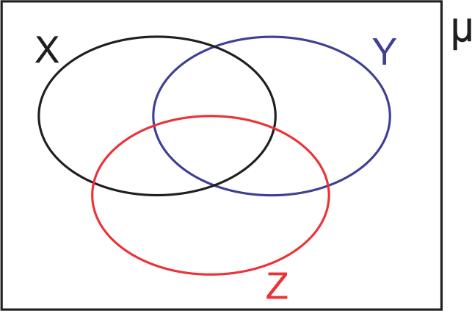
\includegraphics[width=0.55\textwidth]{figures/example1-5-blank.png}
\end{center}

$(X \cup Y)'$ represents elements which are not in $X \cup Y$. We use vertical
lines to shade this region:

\begin{center}
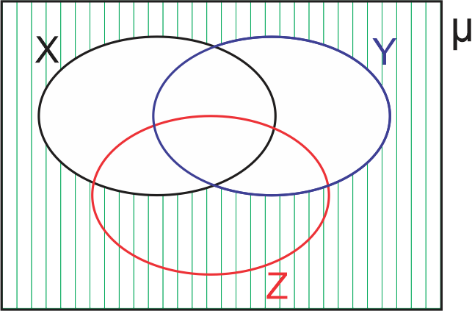
\includegraphics[width=0.55\textwidth]{figures/example1-5-vertical.png}
\end{center}

Then, on the same diagram, set $Z$ is shaded with horizontal lines. The
intersection of $(X \cup Y)'$ and $Z$ is the double-shaded (cross-hatched) area:

\begin{center}
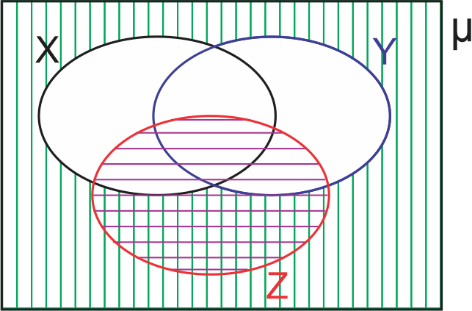
\includegraphics[width=0.55\textwidth]{figures/example1-5-combined.png}
\end{center}

Therefore, $(X \cup Y)' \cap Z$ is the region shown below, shaded in a single
cross-hatch pattern:

\begin{center}
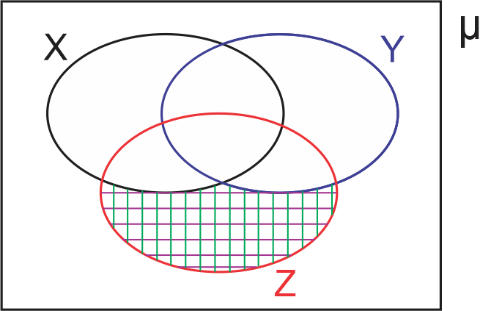
\includegraphics[width=0.55\textwidth]{figures/example1-5-final.png}
\end{center}

\textbf{b. $X' \cap (Y \cup Z)$} is found in the same way: shade $X'$ (everything outside
circle $X$) with vertical lines, shade $Y \cup Z$ with horizontal lines, and the
region shaded by both patterns is the required set.
\end{example}

In year 1, we learned about set theory laws. Examples of these laws include
commutative, associative and distributive. We also learned to identify the regions
in a three-set Venn diagram. In this lesson, we will apply these concepts to answer
real-life problems.

\subsection*{How to complete a three-set Venn diagram}
\begin{enumerate}
  \item Start with the intersection of the three sets and proceed to the regions
  involving two sets.
  \item Then work on the regions involving one set and finally the regions in the
  universal set that do not intersect with any of the three sets.
\end{enumerate}
To summarise, start from the centre (the region with the most overlaps) and work
your way out.

\begin{example}{Example 1.6}
Set $A = \{\text{odd numbers less than } 15\}$

Set $B = \{W : 4 < W \le 11\}$

Set $D = \{\text{Prime numbers less than } 14\}$

All of which are subsets of Set $R = \{0, 1, 2, 3, 4, \ldots, 16\}$.
\begin{enumerate}
  \item[a.] List the members of the following sets: (i) $A$ \quad (ii) $B$ \quad (iii) $D$ \quad (iv) $A \cup B$ \quad (v) $(A \cup B) \cap D'$ \quad (vi) $(A' \cap B) \cup D$.
  \item[b.] Represent $A$, $B$, $D$ and $R$ using a Venn diagram.
\end{enumerate}

\medskip\noindent\textbf{Solution}
\begin{enumerate}
  \item[a.]
  \begin{align*}
    \text{(i)}\quad A &= \{1, 3, 5, 7, 9, 11, 13\} \\
    \text{(ii)}\quad B &= \{5, 6, 7, 8, 9, 10, 11\} \\
    \text{(iii)}\quad D &= \{2, 3, 5, 7, 11, 13\} \\
    \text{(iv)}\quad A \cup B &= \{1, 3, 5, 7, 9, 11, 13\} \cup \{5, 6, 7, 8, 9, 10, 11\} \\
    &= \{1, 3, 5, 6, 7, 8, 9, 10, 11, 13\} \\
    \text{(v)}\quad (A \cup B) \cap D' &= \{1, 3, 5, 6, 7, 8, 9, 10, 11, 13\} \cap \{1, 4, 6, 8, 9, 10, 12, 14, 15, 16\} \\
    &= \{1, 6, 8, 9, 10\} \\
    \text{(vi)}\quad A' \cap B &= \{2, 4, 6, 8, 10, 12, 14, 15, 16\} \cap \{5, 6, 7, 8, 9, 10, 11\} = \{6, 8, 10\} \\
    (A' \cap B) \cup D &= \{6, 8, 10\} \cup \{2, 3, 5, 7, 11, 13\} = \{2, 3, 5, 6, 7, 8, 10, 11, 13\}
  \end{align*}

  \item[b.] We first find the triple intersection: $A \cap B \cap D = \{5, 7, 11\}$.

  \begin{center}
  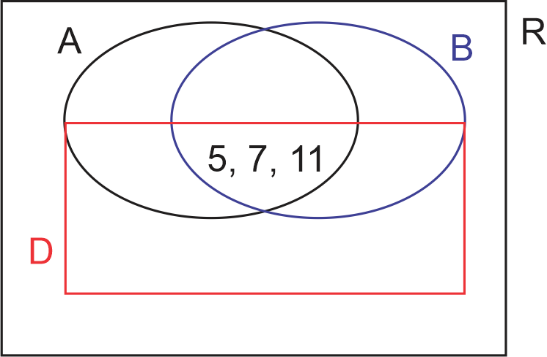
\includegraphics[width=0.55\textwidth]{figures/example1-6-triple.png}
  \end{center}

  Then proceed to the pairwise intersections. There are three of these:
  \begin{align*}
    A \cap B \text{ only} &= A \cap B \cap D' = \{9\} \\
    A \cap D \text{ only} &= A \cap B' \cap D = \{3, 13\} \\
    B \cap D \text{ only} &= A' \cap B \cap D = \{\ \}
  \end{align*}
  Let's update our diagram with these values:

  \begin{center}
  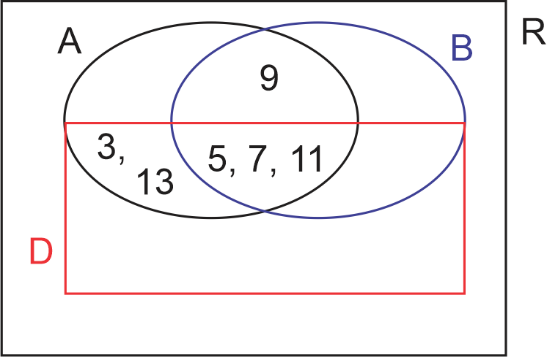
\includegraphics[width=0.55\textwidth]{figures/example1-6-pairwise.png}
  \end{center}

  Next, find the single intersections. There are three of them:
  \begin{align*}
    A \text{ only} &= \{1\} \\
    B \text{ only} &= \{6, 8, 10\} \\
    D \text{ only} &= \{2\}
  \end{align*}

  \begin{center}
  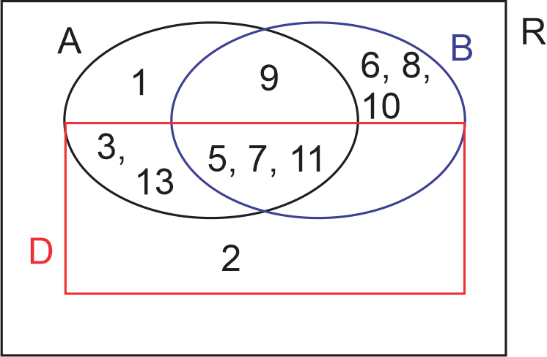
\includegraphics[width=0.55\textwidth]{figures/example1-6-singles.png}
  \end{center}

  Finally, we find $(A \cup B \cup D)' = \{0, 4, 12, 14, 15, 16\}$.

  Find below the completed diagram:
  \begin{center}
  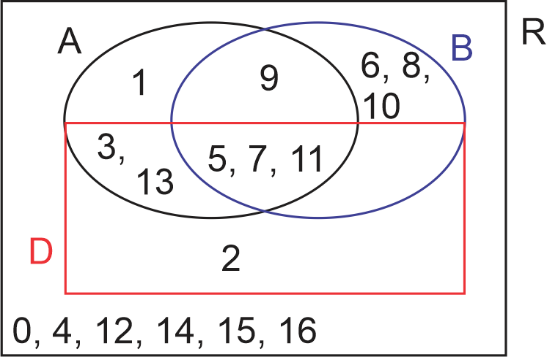
\includegraphics[width=0.55\textwidth]{figures/example1-6-completed.png}
  \end{center}
\end{enumerate}
\end{example}

\begin{example}{Example 1.7}
A survey of 70 investors reveals the following: 30 invest in bonds, 40 in stocks
and 21 in annuities. 10 had investments in bonds and annuities, 15 in bonds and
stocks, 12 in stocks and annuities, and 7 had investments in all three assets. The
remaining investors had investments in other assets.

Create a Venn diagram for this information.

\medskip\noindent\textbf{Solution}

First, draw a Venn diagram with three intersecting sets representing the three
main sets: Bonds, Stocks, and Annuities. Let $B$ represent Bonds, $A$ represent
Annuities and $S$ represent Stocks. This means $n(B) = 30$, $n(A) = 21$ and
$n(S) = 40$.

\begin{center}
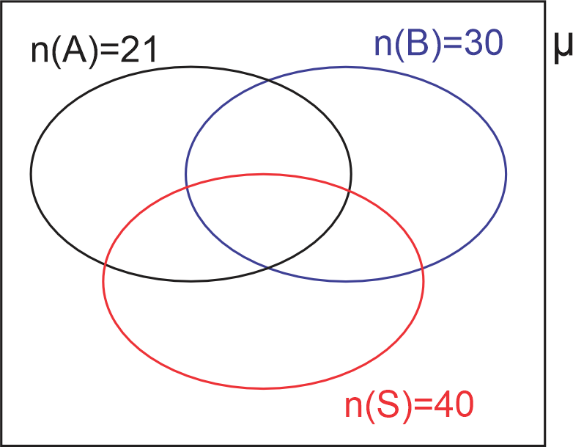
\includegraphics[width=0.5\textwidth]{figures/example1-7-blank.png}
\end{center}

Next, we fill in the region where all three sets intersect. From the question,
this figure is 7.

\begin{center}
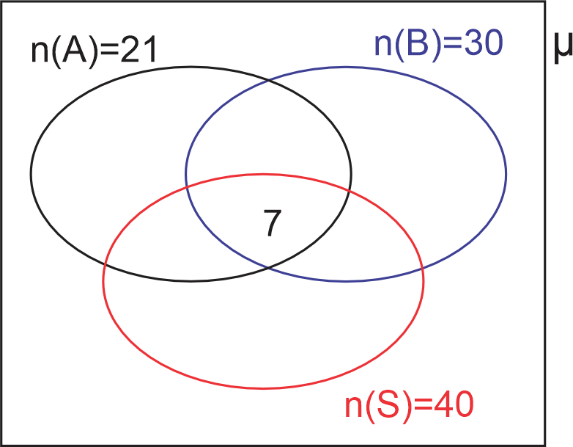
\includegraphics[width=0.5\textwidth]{figures/example1-7-triple.png}
\end{center}

Let us add these values to the Venn diagram. Next, we fill in the regions where
exactly two sets intersect:
\begin{enumerate}
  \item[a.] \textbf{Bonds and Annuities.} A total of 10 had investments in bonds and
  annuities but 7 of them have investments in all three assets. This leaves
  $10 - 7 = 3$ investing in only Bonds and Annuities.
  \item[b.] \textbf{Bonds and Stocks.} A total of 15 had investments in bonds and
  stocks but 7 of them had investments in all three assets. This leaves
  $15 - 7 = 8$ investing in only Bonds and Stocks.
  \item[c.] \textbf{Stocks and Annuities.} A total of 12 had investments in stocks and
  annuities but 7 of them have investments in all three assets. This leaves
  $12 - 7 = 5$ investing in only Stocks and Annuities.
\end{enumerate}

\begin{center}
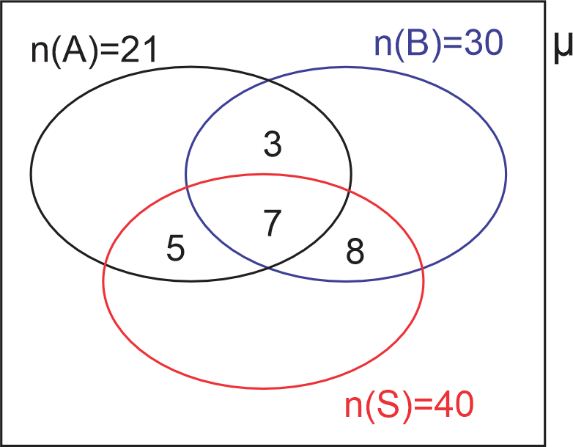
\includegraphics[width=0.5\textwidth]{figures/example1-7-pairwise.png}
\end{center}

You will realise there is only one region remaining in each set. These are the
regions that represent only one set:
\begin{enumerate}
  \item[a.] \textbf{Only Bonds.} A total of 30 had investments in bonds but we have
  already accounted for $3 + 7 + 8 = 18$ of them, leaving $30 - 18 = 12$ having
  investments in only Bonds.
  \item[b.] \textbf{Only Annuities.} A total of 21 had investments in annuities but we
  have already accounted for $3 + 7 + 5 = 15$ of them, leaving $21 - 15 = 6$
  having investments in only Annuities.
  \item[c.] \textbf{Only Stocks.} A total of 40 had investments in stocks but we have
  already accounted for $5 + 7 + 8 = 20$ of them, leaving $40 - 20 = 20$
  investing in only Stocks.
\end{enumerate}

We will add these values to the Venn diagram:

\begin{center}
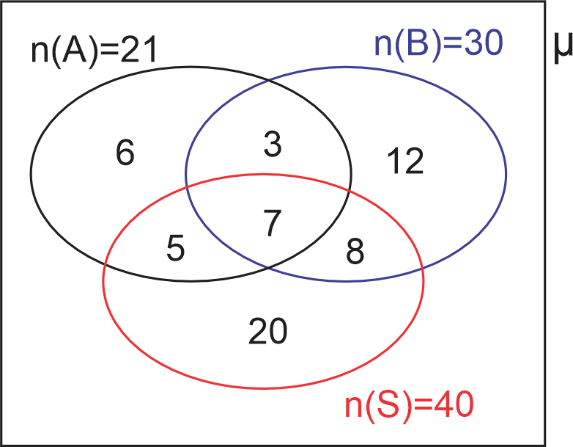
\includegraphics[width=0.5\textwidth]{figures/example1-7-singles.png}
\end{center}

Finally, we calculate the number of investors with no investments in the three
assets. The sum of all the values already calculated for the intersecting sets is
\[
  12 + 3 + 6 + 8 + 5 + 7 + 20 = 61.
\]
This means $70 - 61 = 9$ investors did not invest in any of the three assets. This
value is recorded outside the circles but inside the universal set, completing the
Venn diagram:

\begin{center}
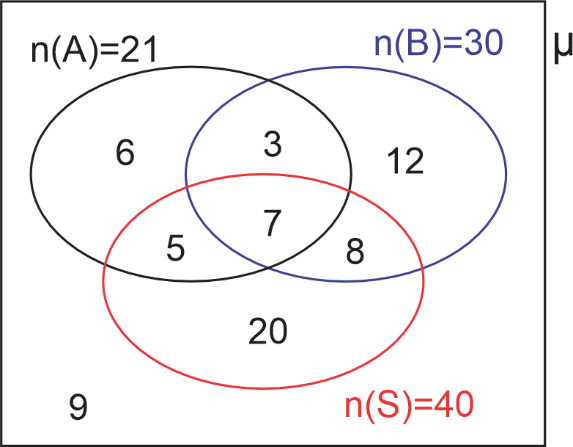
\includegraphics[width=0.55\textwidth]{figures/example1-7-completed.png}
\end{center}
\end{example}

\begin{example}{Example 1.8}
A survey of 97 countries that participated in the Olympics reveals that 80 won
bronze, 57 won silver and 47 won gold. It also reveals that 30 won gold and
silver, 50 won silver and bronze, 38 won gold and bronze, and 3 countries did not
win any medal.
\begin{enumerate}
  \item[a.] Illustrate the information on a Venn diagram.
  \item[b.] Calculate the number of countries who won all three medals.
  \item[c.] Calculate the number of countries who won exactly two medals.
\end{enumerate}

\medskip\noindent\textbf{Solution}

Let $B$ = Bronze medal, $G$ = Gold medal, and $S$ = Silver medal, so
$n(B) = 80$, $n(S) = 57$ and $n(G) = 47$.

Let $x$ be the number of countries who won all three medals (unknown, since we
were not given this directly).

\begin{center}
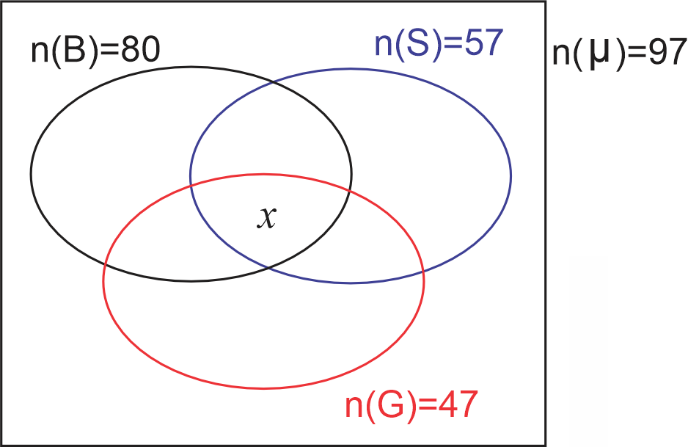
\includegraphics[width=0.5\textwidth]{figures/example1-8-blank.png}
\end{center}

Next, we fill in the regions where exactly two sets intersect (countries that won
exactly two of the three medals). A total of 30 countries won Gold and Silver;
of these, $x$ won all three medals, so $(30-x)$ countries won \emph{only} Gold and
Silver. Similarly, 50 won Silver and Bronze, giving $(50 - x)$ who won only
Silver and Bronze, and 38 won Gold and Bronze, giving $(38-x)$ who won only
Gold and Bronze.

\begin{center}
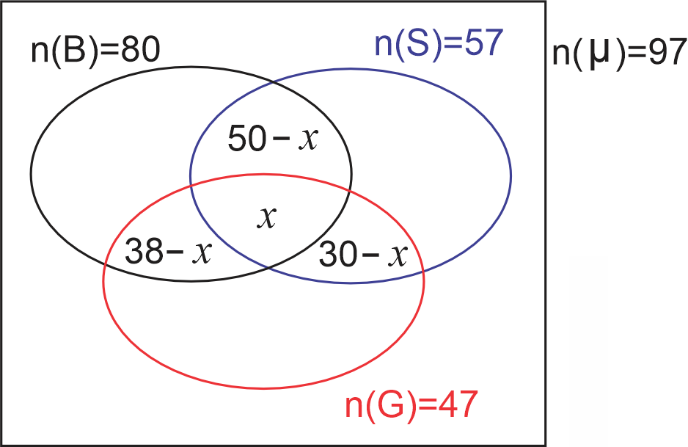
\includegraphics[width=0.5\textwidth]{figures/example1-8-pairwise.png}
\end{center}

At this point only one region remains in each set:
\begin{itemize}
  \item \textbf{Only Bronze.} $80$ won bronze, and we have already accounted for
  $x + (50-x) + (38-x) = (88-x)$ of them, leaving $80 - (88-x) = (x - 8)$
  winning only bronze.
  \item \textbf{Only Silver.} $57$ won silver, and we have already accounted for
  $x + (50-x) + (30-x) = (80-x)$ of them, leaving $57 - (80-x) = (x - 23)$
  winning only silver.
  \item \textbf{Only Gold.} $47$ won gold, and we have already accounted for
  $x + (30-x) + (38-x) = (68-x)$ of them, leaving $47 - (68-x) = (x - 21)$
  winning only gold.
\end{itemize}

\begin{center}
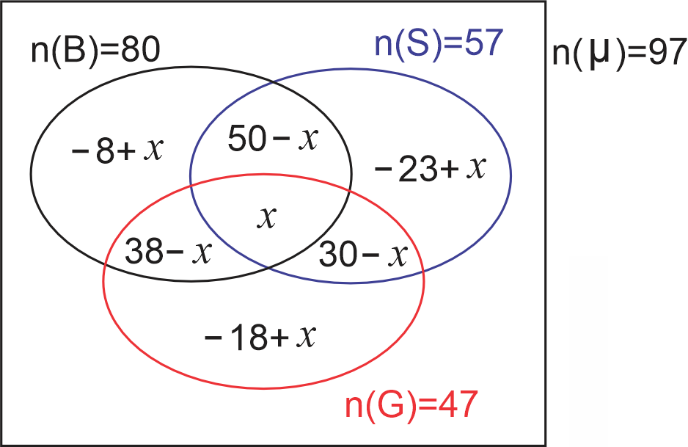
\includegraphics[width=0.5\textwidth]{figures/example1-8-singles.png}
\end{center}

\textit{(Note: the Gold-only region in this diagram is labelled $-18+x$ in the
original textbook figure --- this is a typo. As derived above, the correct
formula is $x-21$. We use the correct formula going forward.)}

According to the question, 3 countries did not win any medal, so
$(G \cup S \cup B)' = 3$.

\begin{center}
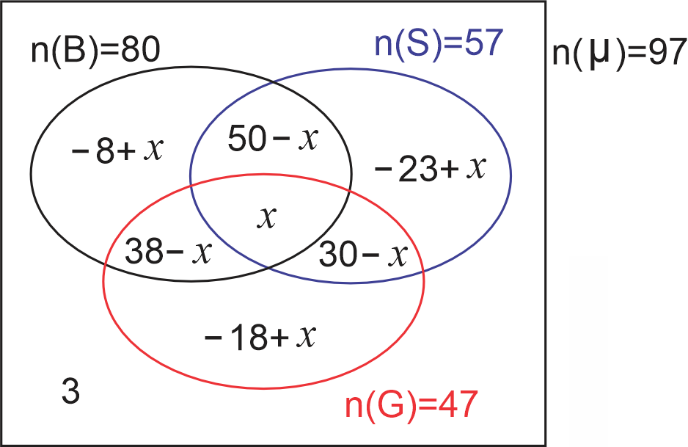
\includegraphics[width=0.5\textwidth]{figures/example1-8-nomedal.png}
\end{center}

To solve for $x$, add all the entries and equate the result to the total number of
countries under consideration (97):
\[
  x + (30-x) + (50-x) + (38-x) + (x-8) + (x-23) + (x-21) + 3 = 97
\]
\[
  x + 69 = 97 \implies x = 97 - 69 = 28.
\]

\begin{enumerate}
  \item[e.] Therefore, \textbf{28} countries won all three medals.
  \item[f.] Number of countries that won exactly two medals $= (30-28) + (50-28) + (38-28) = 2 + 22 + 10 = 34$.
\end{enumerate}

We can now update the diagram with this value. The completed Venn diagram, as
given in the original textbook, is:
\begin{center}
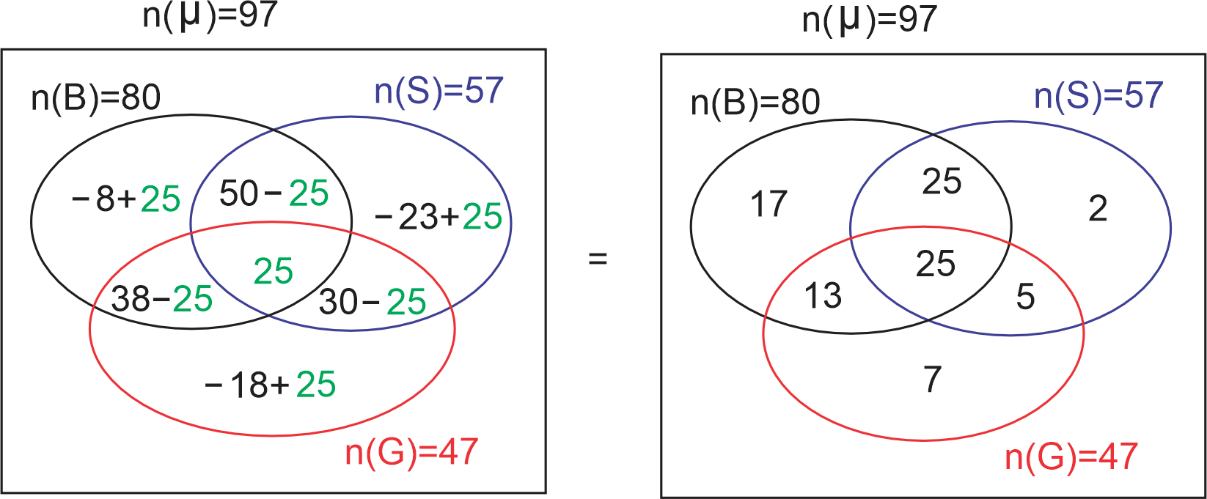
\includegraphics[width=0.85\textwidth]{figures/example1-8-final-book.png}
\end{center}

\textit{Important note:} the textbook substitutes $x=25$ into the region
formulas above, not the value $x=28$ that was just solved for algebraically.
This is an error in the original --- every region value shown (17, 25, 2, 13,
25, 5) other than the Gold-only region is inconsistent with $x=28$, and the
diagram's own values do not agree with part (f)'s answer of 34 for the number
of countries winning exactly two medals ($25+13+5=43\neq34$, using the
diagram's own printed numbers). Substituting the correctly-solved $x=28$
into each formula instead gives Bronze-only $=x-8=20$,
Bronze$\cap$Silver-only $=50-x=22$, Silver-only $=x-23=5$,
Bronze$\cap$Gold-only $=38-x=10$, Silver$\cap$Gold-only $=30-x=2$, and
Gold-only $=x-21=7$ (triple intersection $=28$), which does check against
part (f): $2+22+10=34$.
\end{example}
